\chapter{Results of experiments with \grp}
\label{app:grp}
\textit{This Appendix, presents graphically a summary of individuals runs using \grp. Figures show a \textit{box-plot} representation for different strategies and a bar representation for the percentage of winner solvers types.}
\vfill
\newpage

In Figures~\ref{boxplot:834comm}, \ref{boxplot:1055comm} and \ref{boxplot:1172comm}, labels of the x-axis correspond to the following strategies:
\begin{enumerate}[itemsep=-1mm]
\item \textbf{NC(noT)}: Non communication strategy without using tabu list, 
\item \textbf{NC(T)}: Non communication strategy using tabu list,
\item \textbf{C1-1}: Communicating solvers performing communication \oneTone,
\item \textbf{C1-n}: Communicating solvers performing communication \oneTn.
\end{enumerate}

Figures~\ref{barplot:834}, \ref{barplot:1055} and \ref{barplot:1172}, represent the percentage of winner solvers for each communication strategy, according to four different types:
\begin{enumerate}[itemsep=-1mm]
\item \receiver{Receiver}: Receiver solver wining thanks to the received information, 
\item \sender{Sender}: Sender solver, 
\item \nonreceiver{Pasive receiver}: Receiver solver wining without using the received information,
\end{enumerate}

\begin{figure}[!h]
\centering
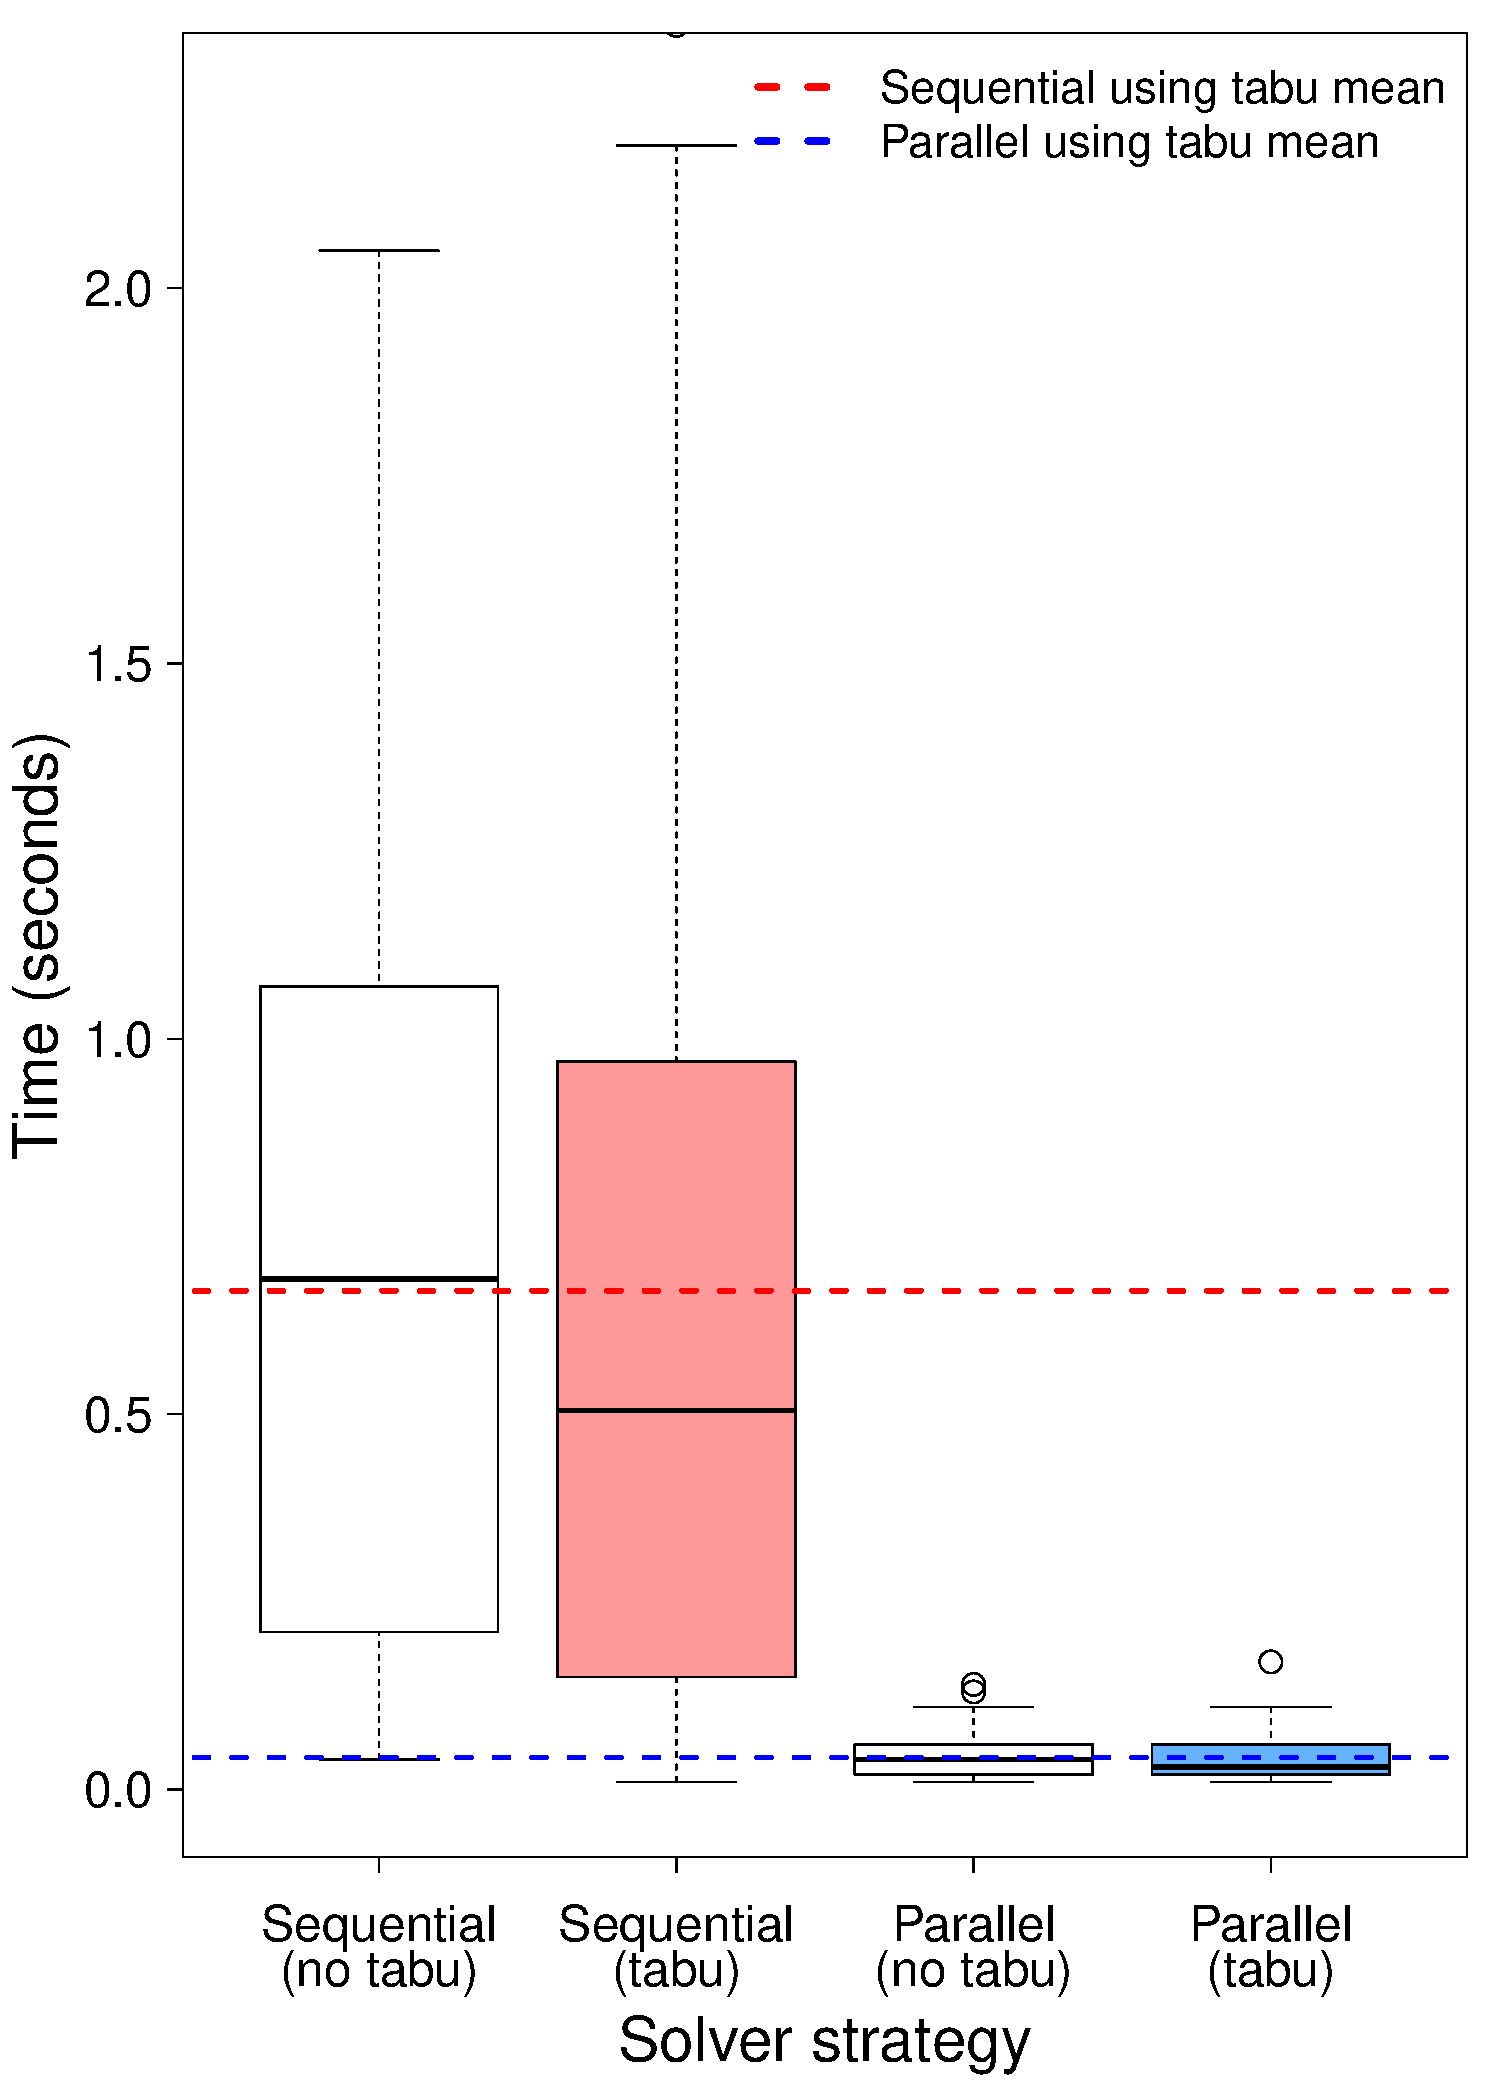
\includegraphics[width=0.8\textwidth]{gol8_select_BP.pdf}
\caption{Comparison between sequential and parallel runs to solve \GRP{} 8-34 using \posl}
\end{figure}

\begin{figure}[!h]
\centering
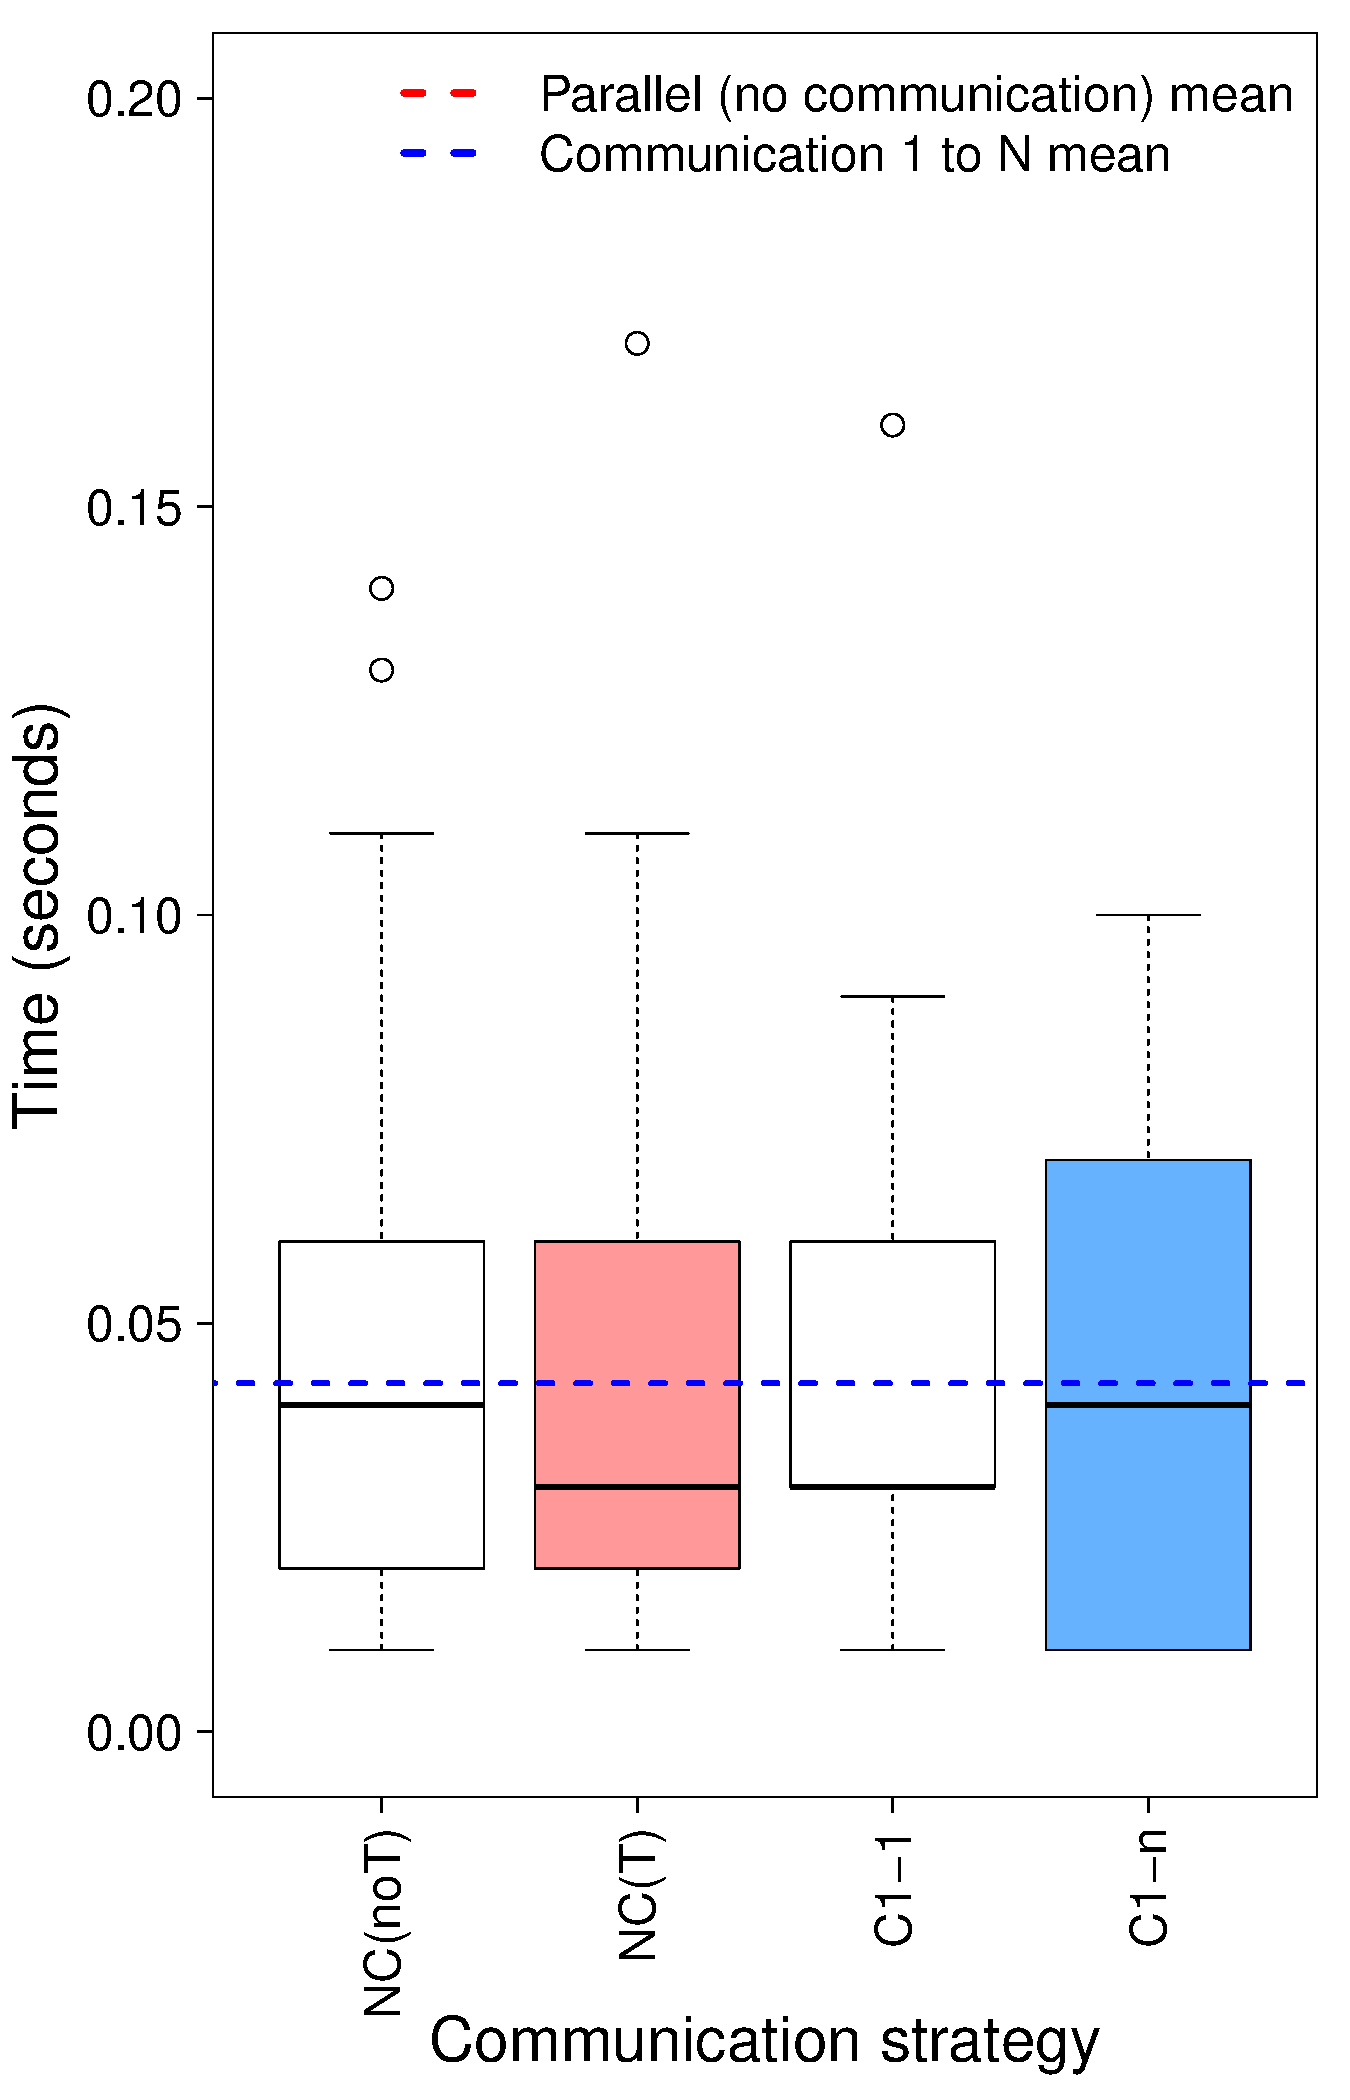
\includegraphics[width=0.8\textwidth]{gol8_comm_BP.pdf}
\caption{Different communication strategies to solve \GRP{} 8-34 using \posl}\label{boxplot:834comm}
\end{figure}

\begin{figure}[!h]
\centering
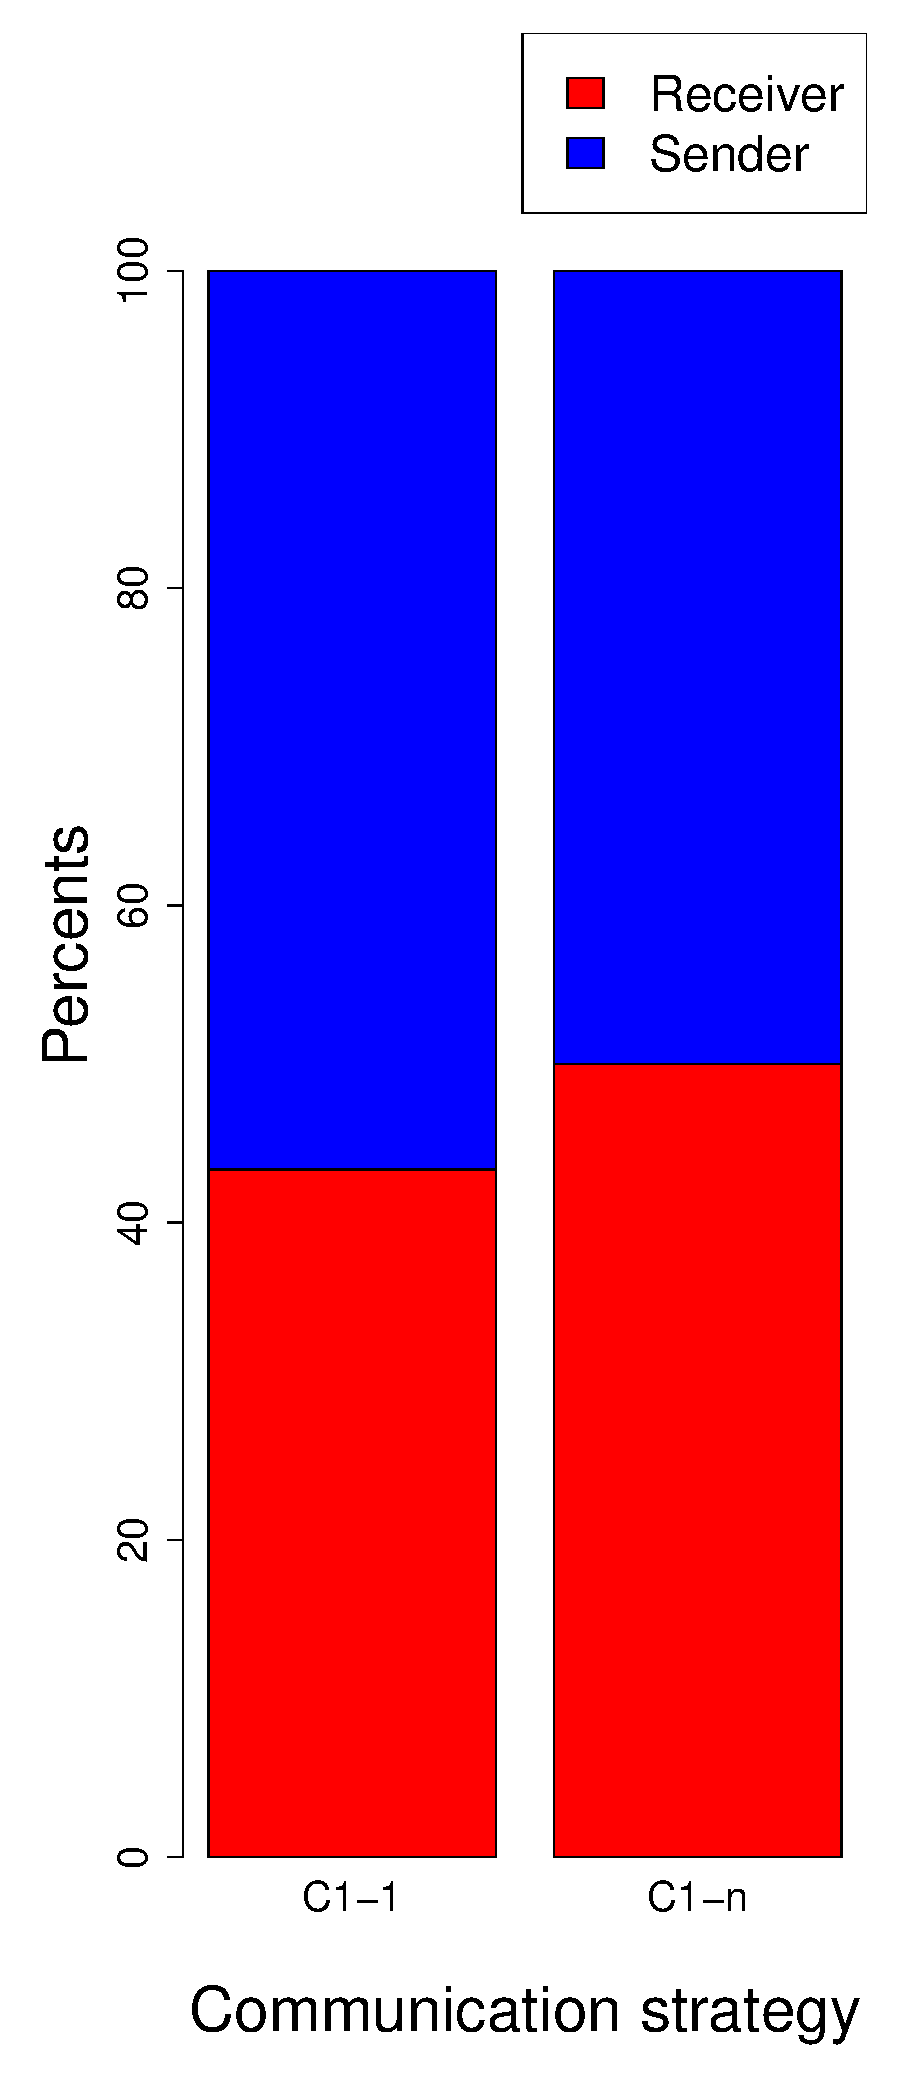
\includegraphics[width=0.8\textwidth]{gol8_per_BP.pdf}
\caption{Solver proportion for each communication strategy to solve \GRP{} 834 using \posl}\label{barplot:834}
\end{figure}

%--------------------------------------

\begin{figure}[!h]
\centering
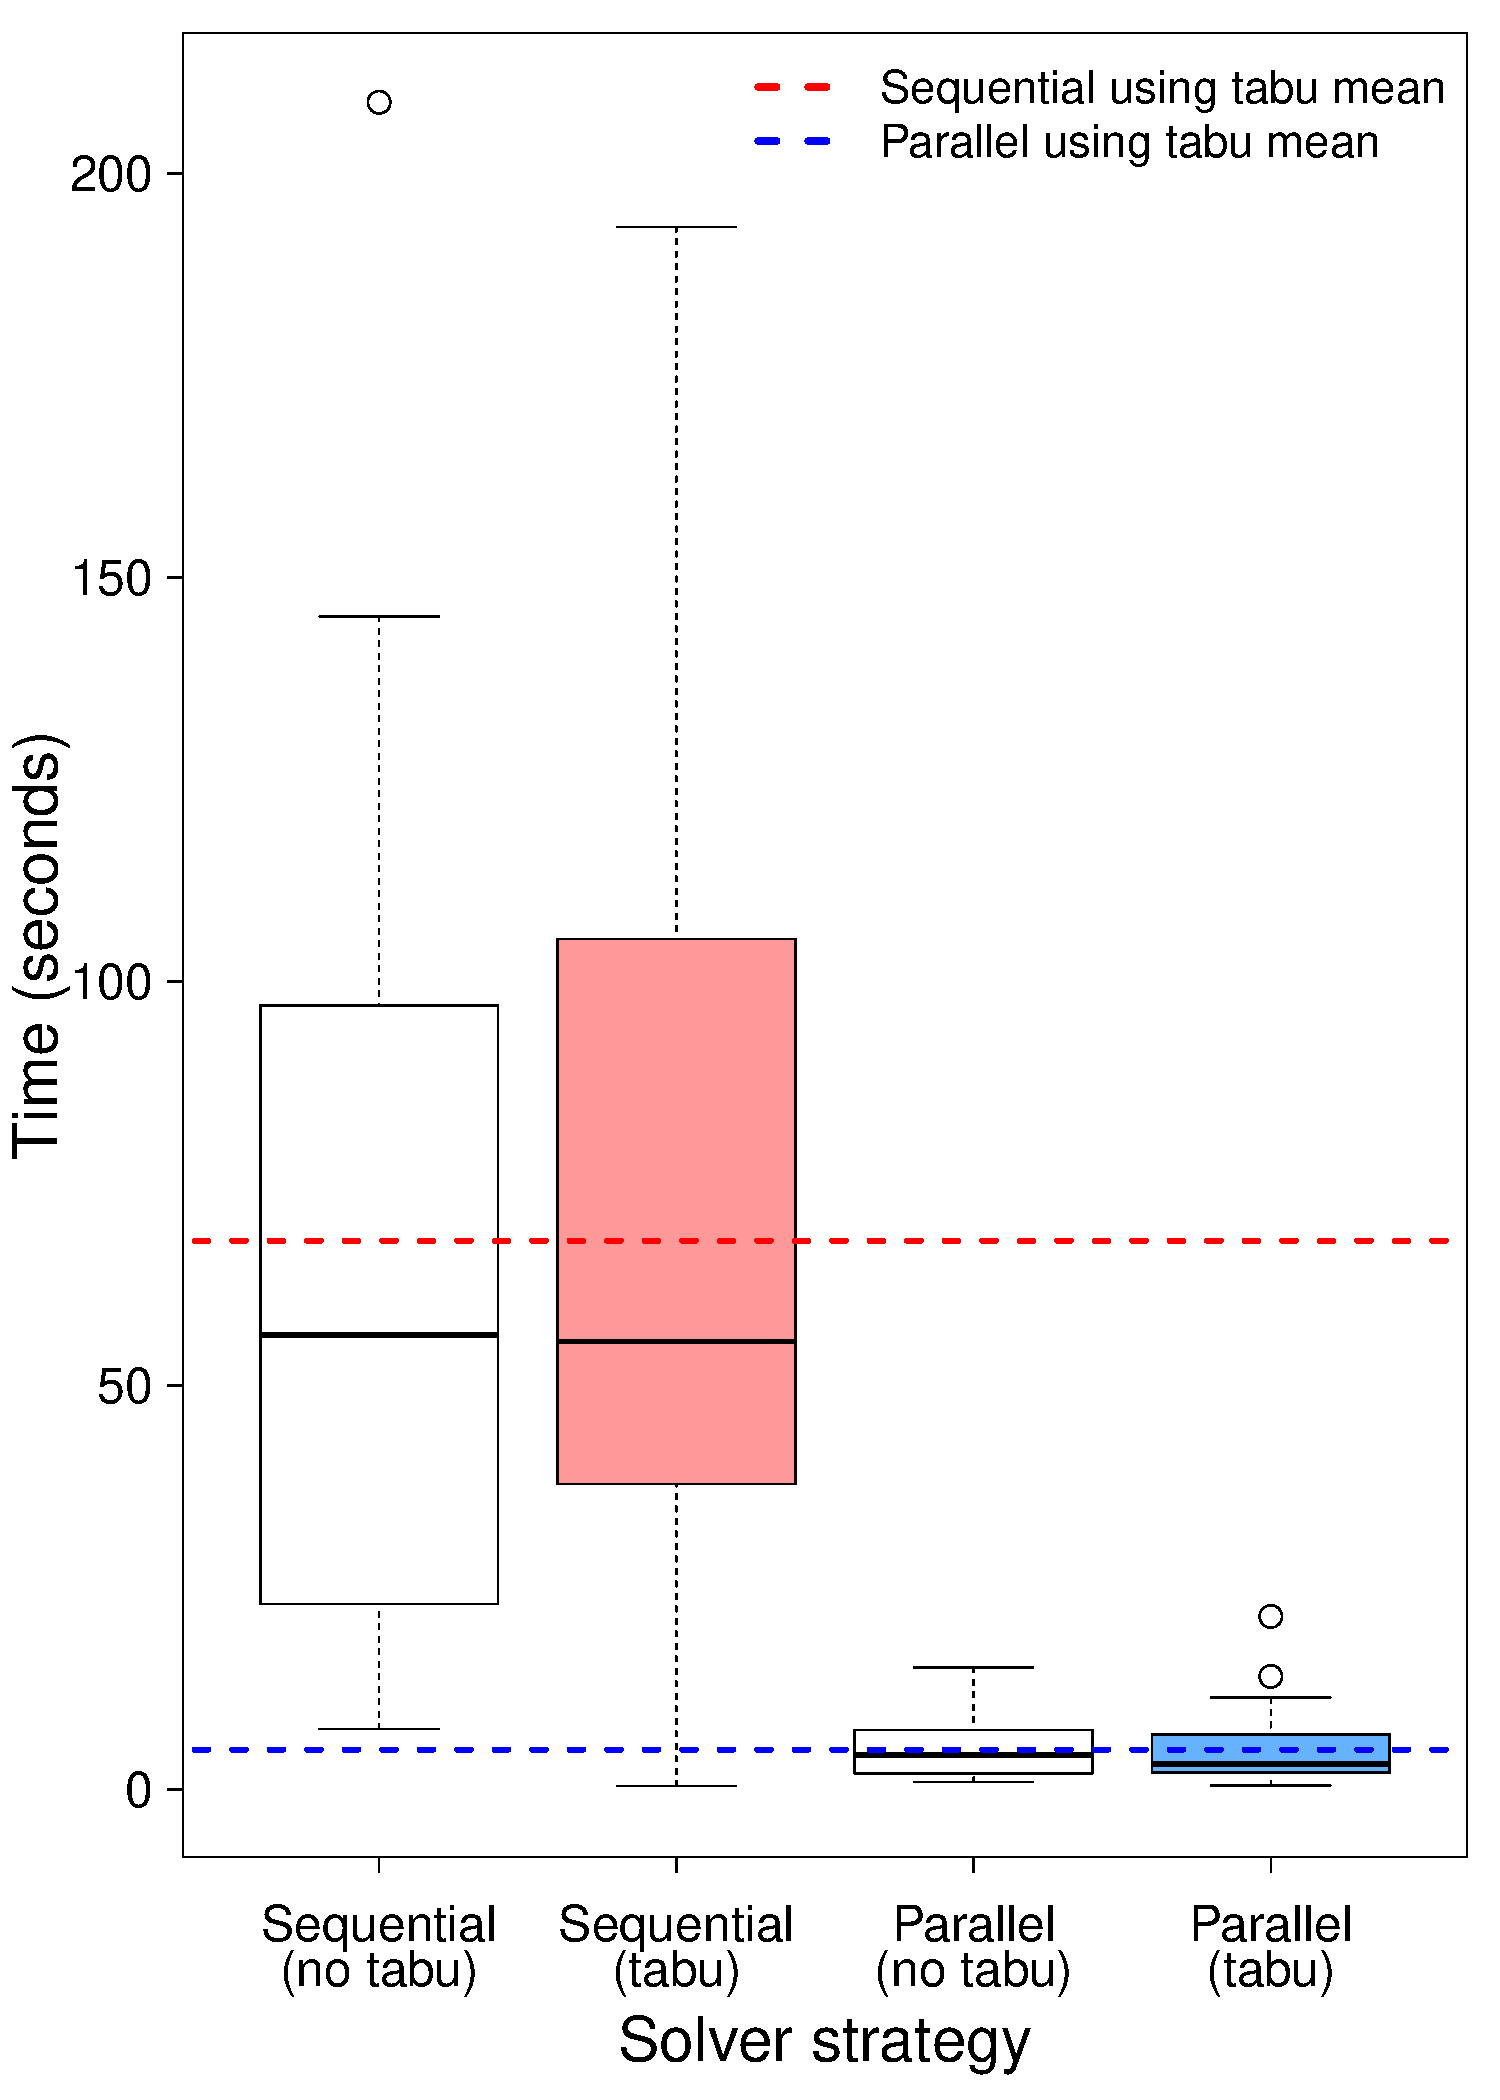
\includegraphics[width=0.75\textwidth]{gol10_select_BP.pdf}
\caption{Comparison between sequential and parallel runs to solve \GRP{} 10-55 using \posl}
\end{figure}

\begin{figure}[!h]
\centering
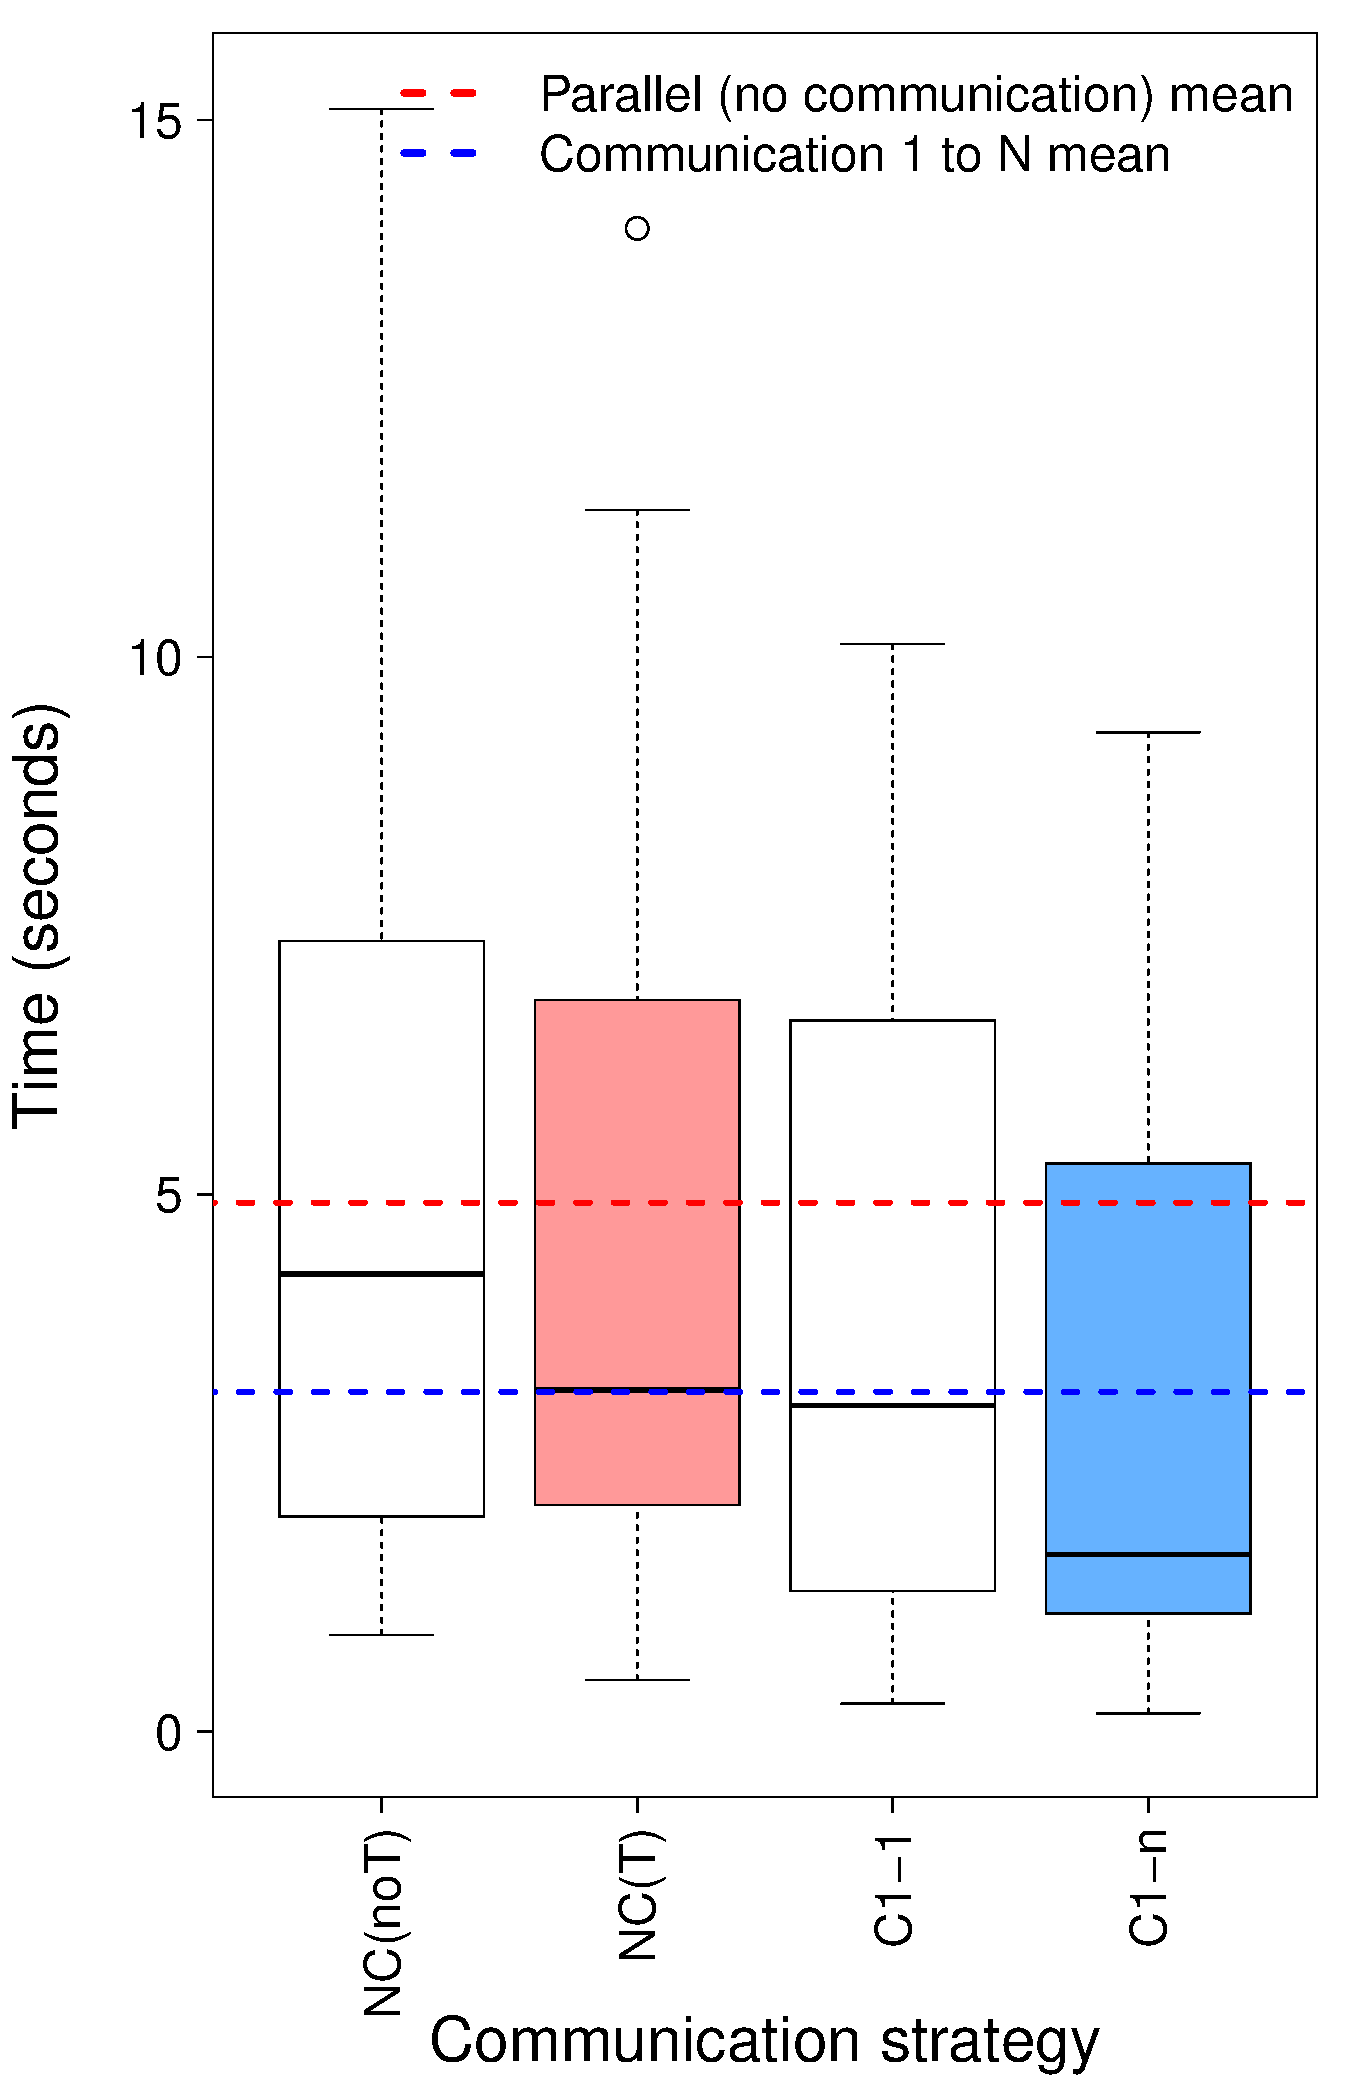
\includegraphics[width=0.75\textwidth]{gol10_comm_BP.pdf}
\caption{Different communication strategies to solve \GRP{} 10-55 using \posl}\label{boxplot:1055comm}
\end{figure}

\begin{figure}[!h]
\centering
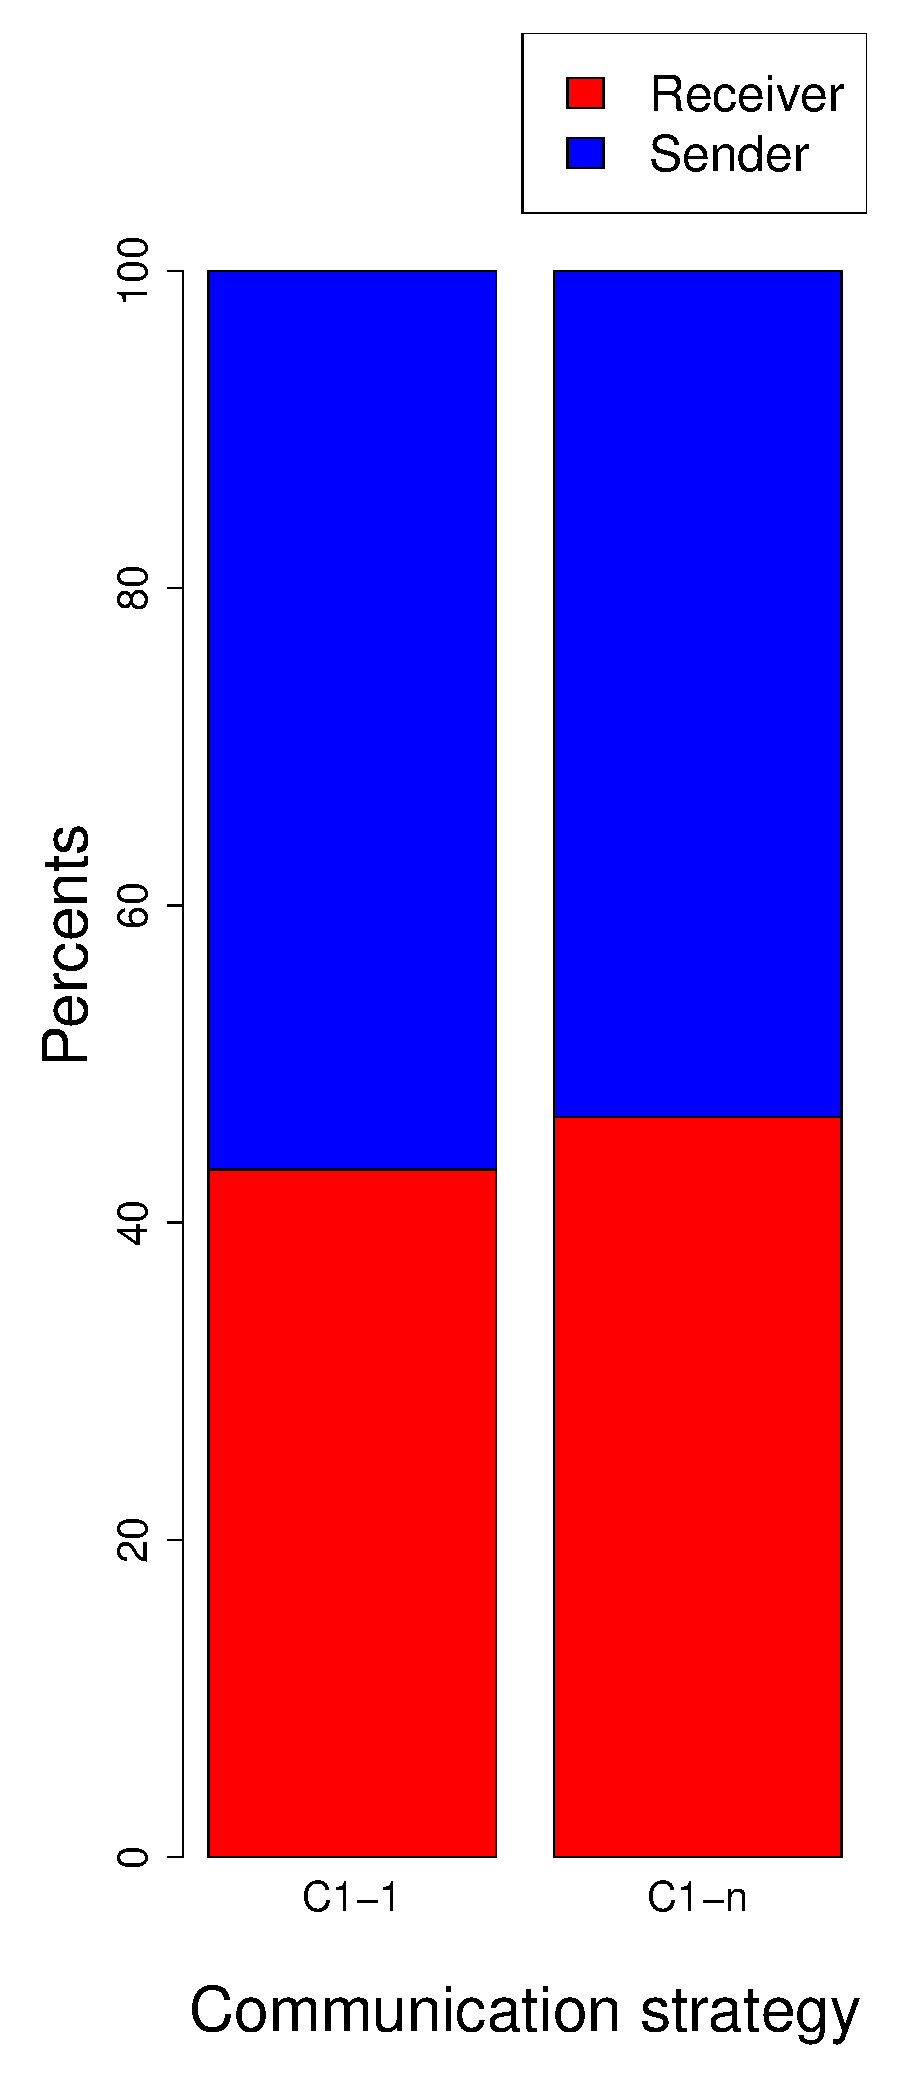
\includegraphics[width=0.8\textwidth]{gol10_per_BP.pdf}
\caption{Solver proportion for each communication strategy to solve \GRP{} 10-55 using \posl}\label{barplot:1055}
\end{figure}

%--------------------------------------

\begin{figure}[!h]
\centering
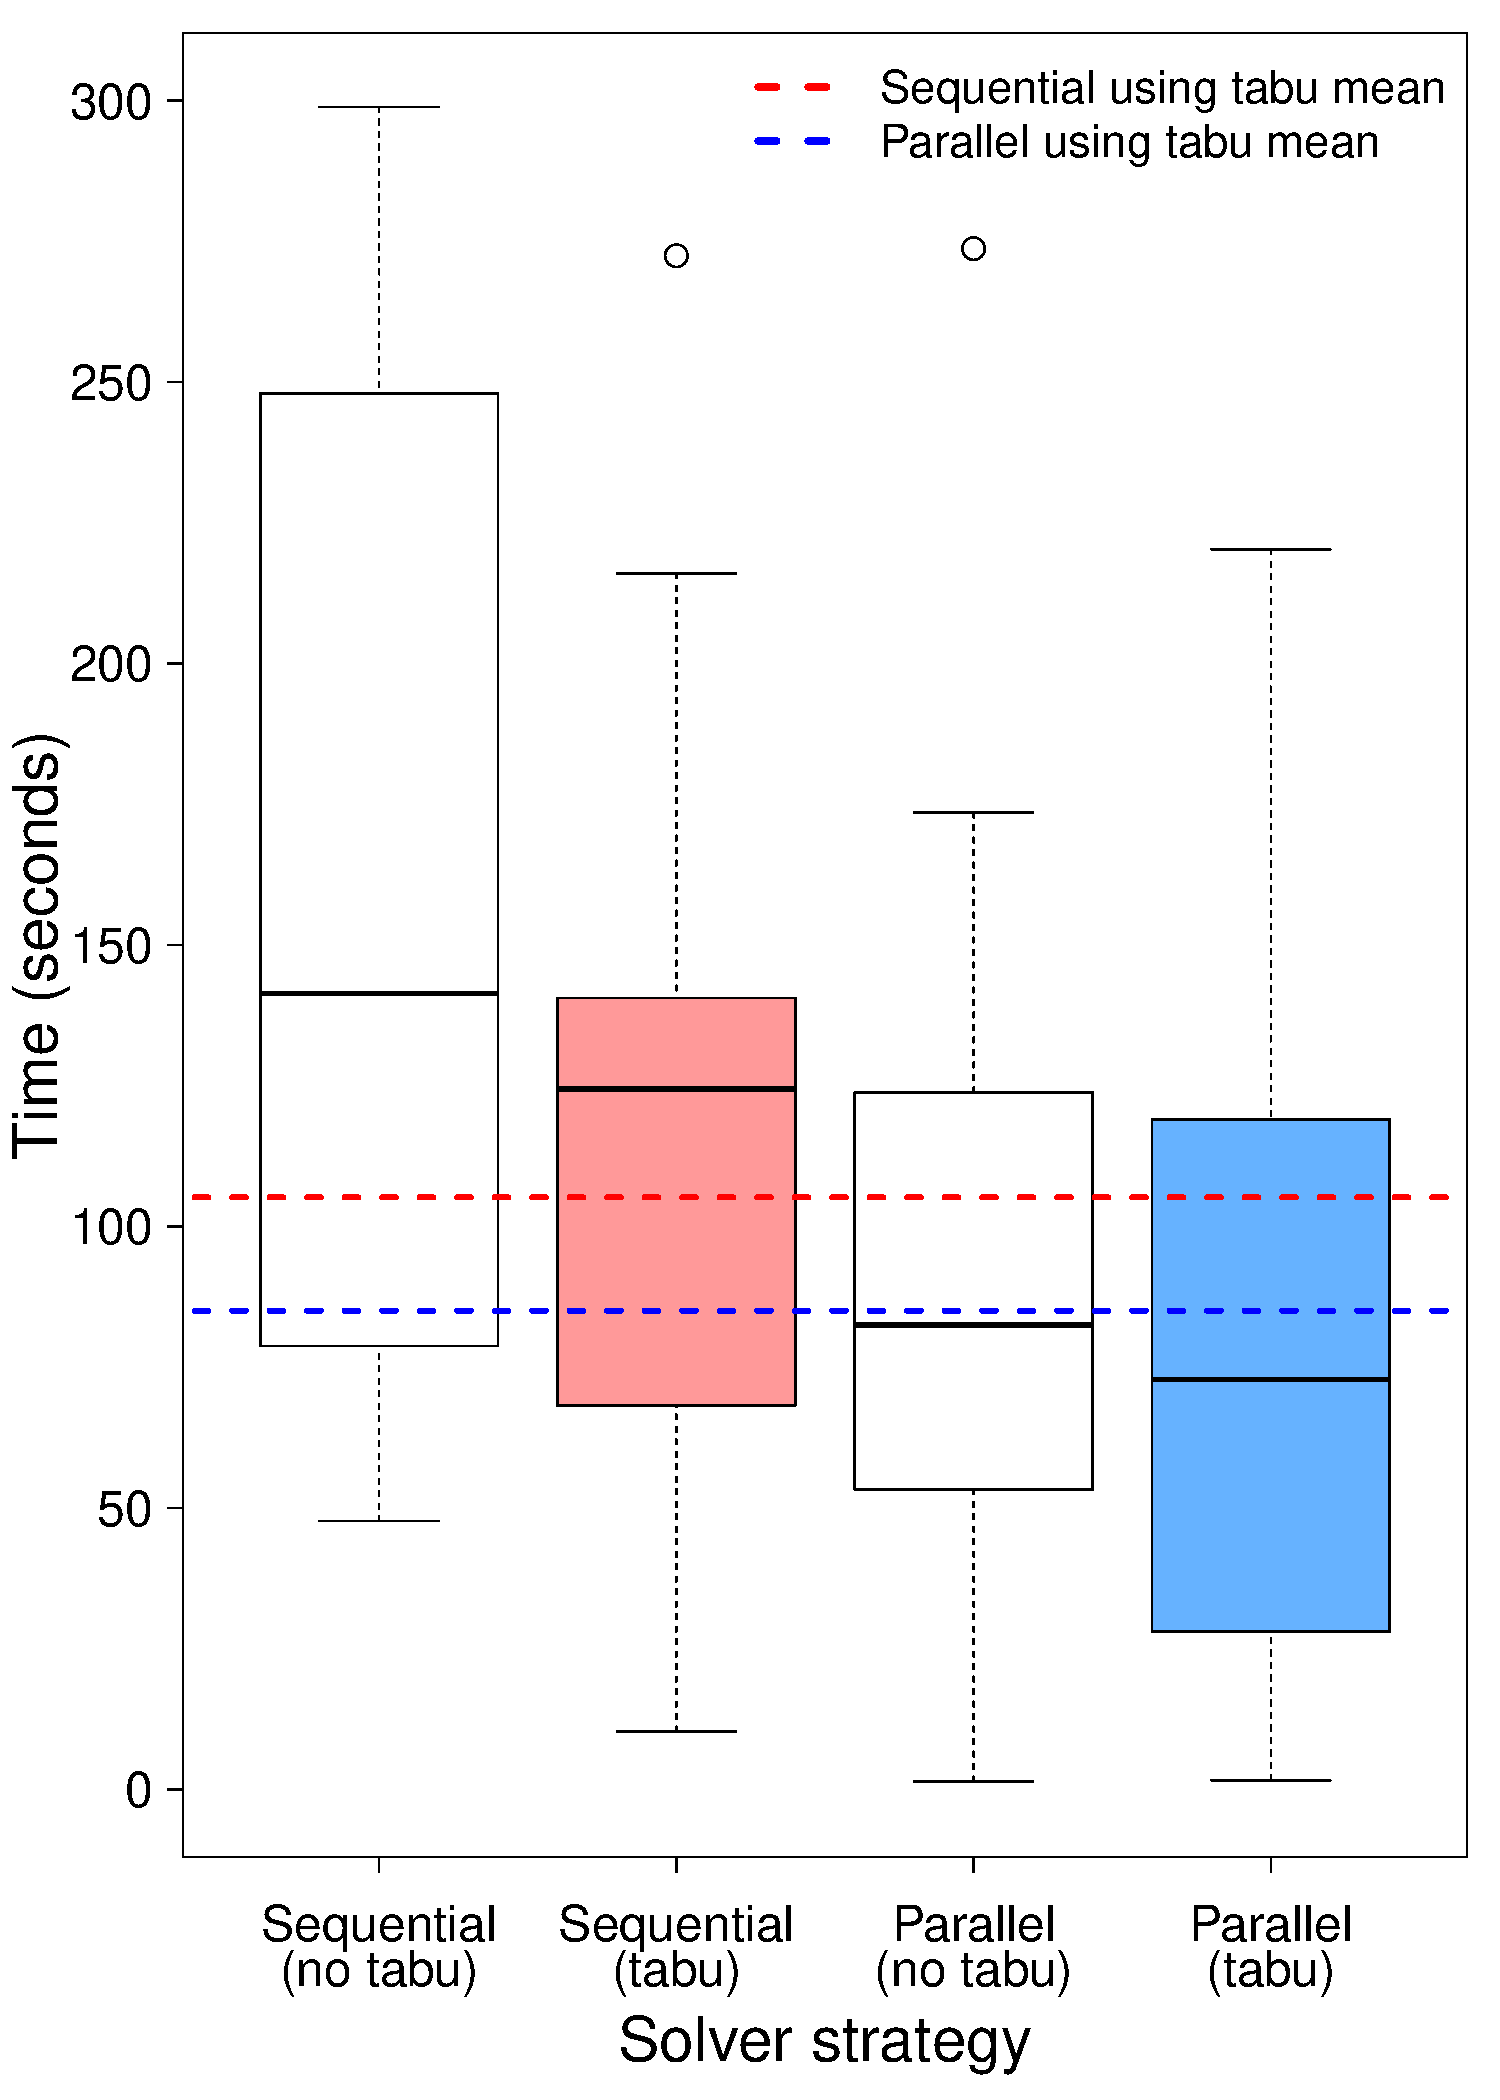
\includegraphics[width=0.75\textwidth]{gol11_select_BP.pdf}
\caption{Comparison between sequential and parallel runs to solve \GRP{} 11-72 using \posl}
\end{figure}

\begin{figure}[!h]
\centering
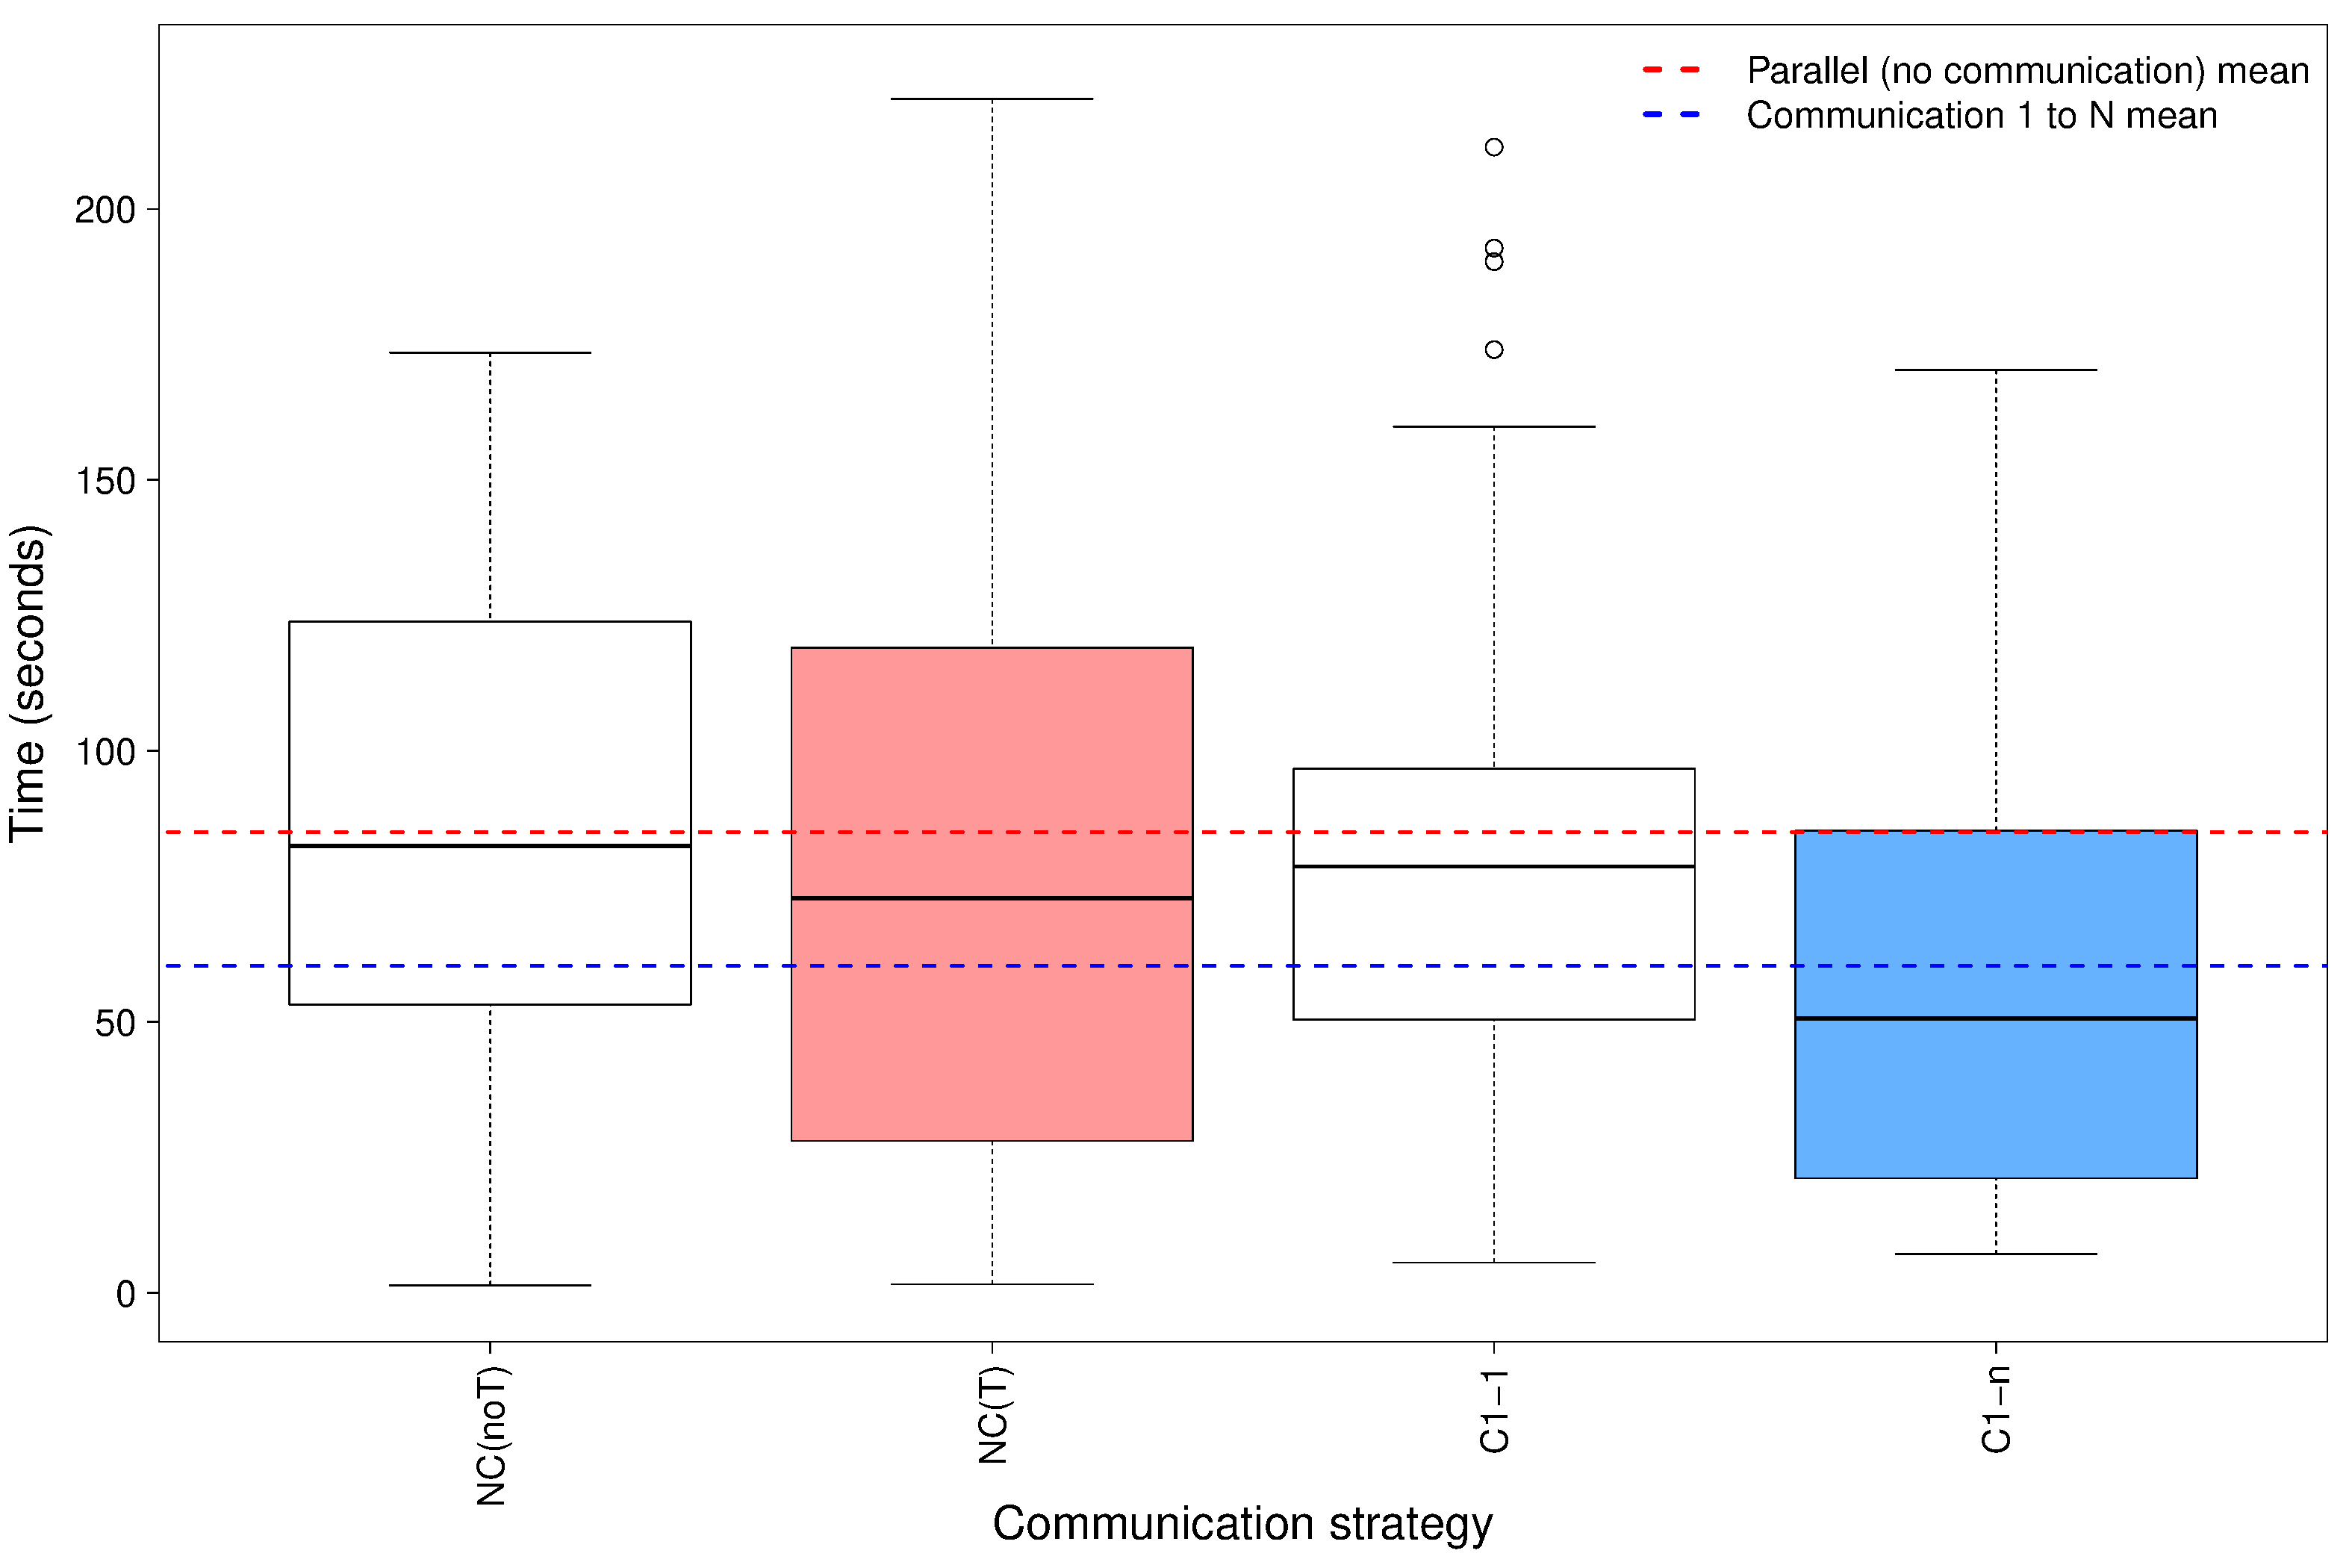
\includegraphics[width=0.75\textwidth]{gol11_comm_BP.pdf}
\caption{Different communication strategies to solve \GRP{} 11-72 using \posl}\label{boxplot:1172comm}
\end{figure}

\begin{figure}[!h]
\centering
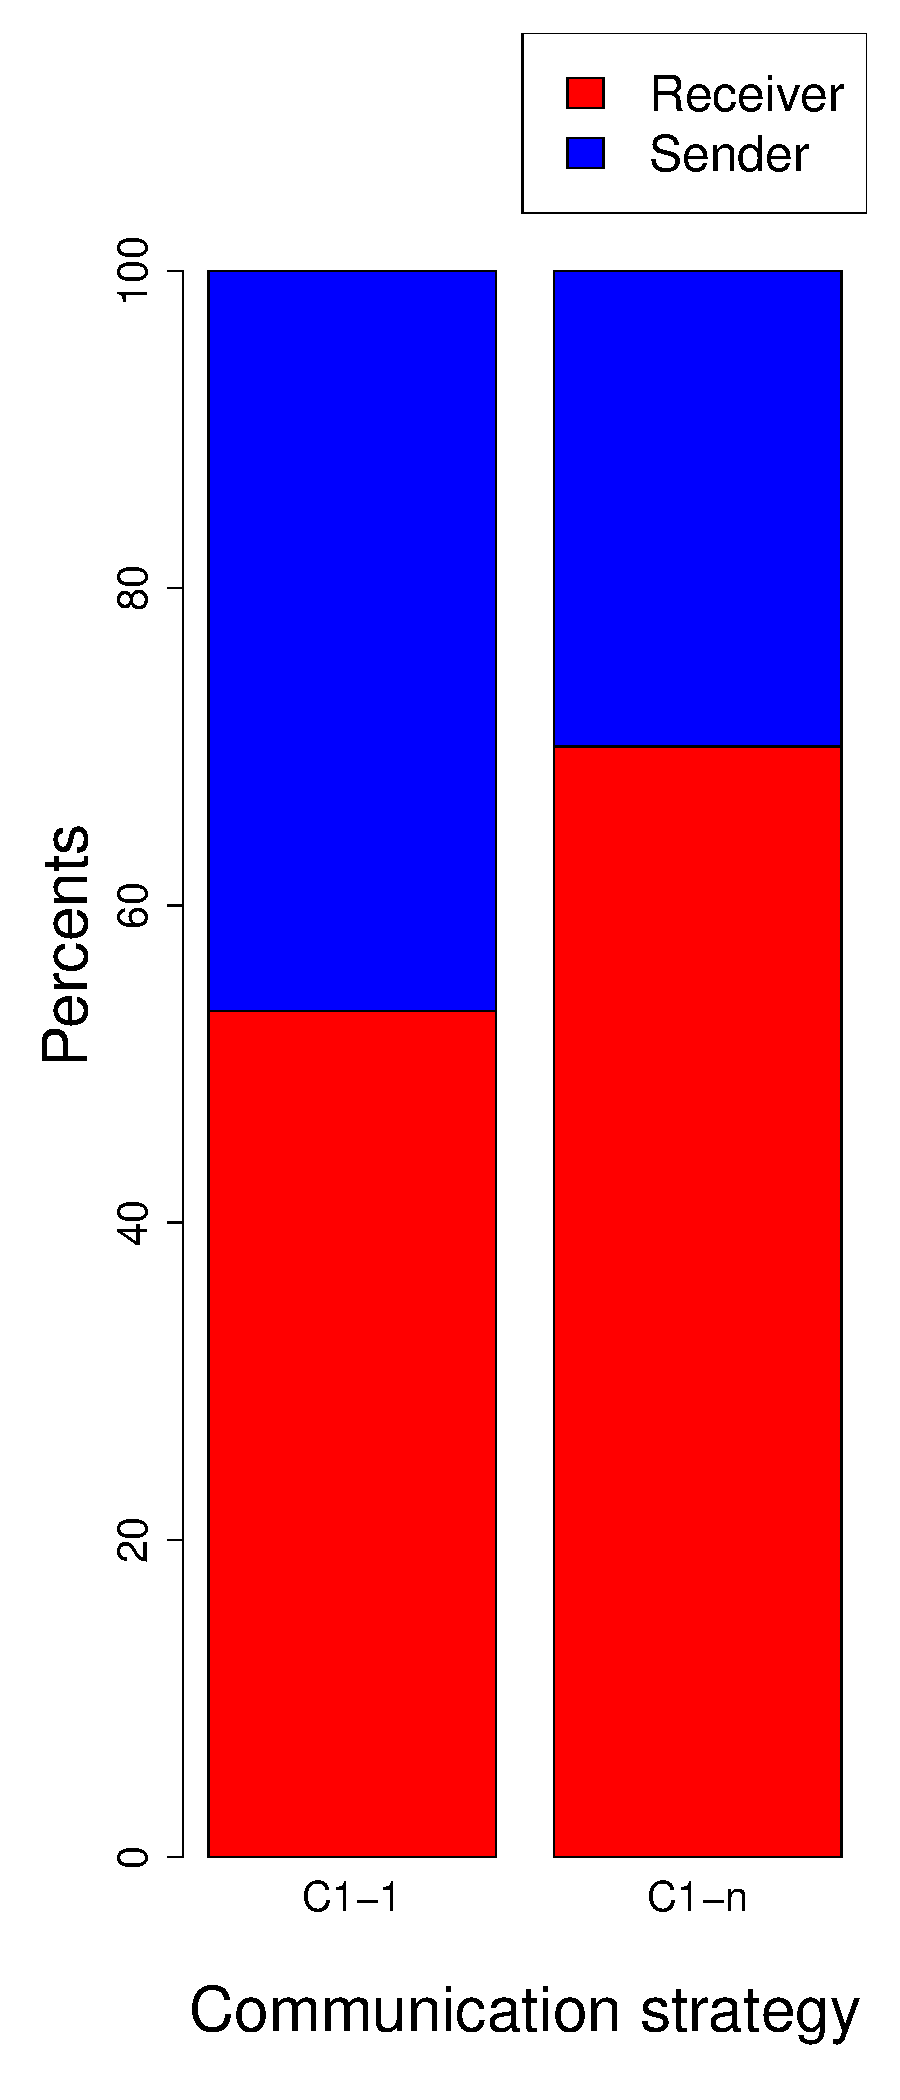
\includegraphics[width=0.8\textwidth]{gol11_per_BP.pdf}
\caption{Solver proportion for each communication strategy to solve \GRP{} 11-72 using \posl}\label{barplot:1172}
\end{figure}